First we plot the original datasets to visualize the data distribution.
The original Vowel dataset is shown in Figure \ref{fig:vowel_dataset}.
The original Mushroom dataset cannot give us meaningful visual information at this time 
since all its features are categorical and one-hot encoded. 

\begin{figure}[h!]
    \centering
    % Segunda subfigura
    \begin{subfigure}[b]{0.45\textwidth}
        \centering
        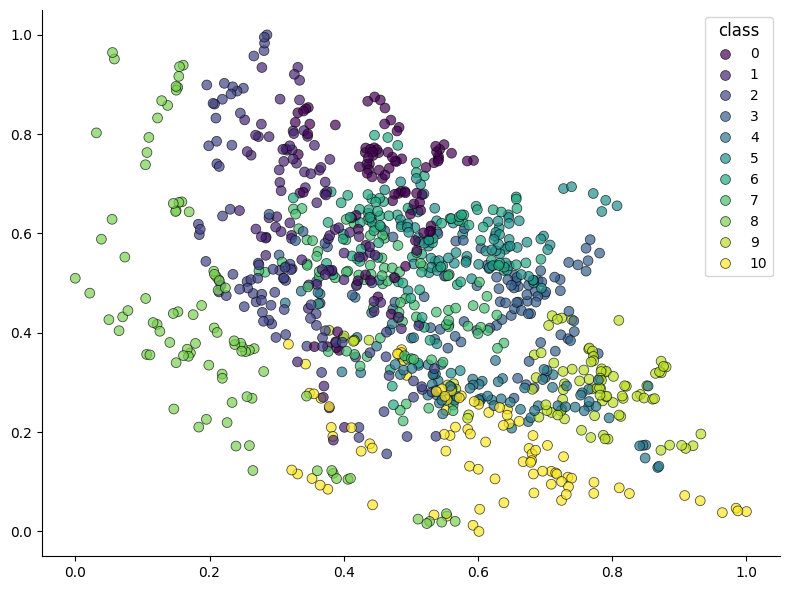
\includegraphics[width=\textwidth]{figures/vowel_dataset.png}
        % \caption{Reduced Vowel dataset}
        \label{Img6}
    \end{subfigure}
    
    \caption{Visualization of the original Vowel dataset}
    \label{fig:vowel_dataset}
\end{figure}

We developed our own implementation of PCA and compared it with several scikit-learn based PCA implementations.
The results of the reduced datasets using our PCA implementation are shown in Figure \ref{fig:our_pca_datasets}.

\begin{figure}[h!]
    \centering
    % Primera subfigura 
    \begin{subfigure}[b]{0.45\textwidth}
        \centering
        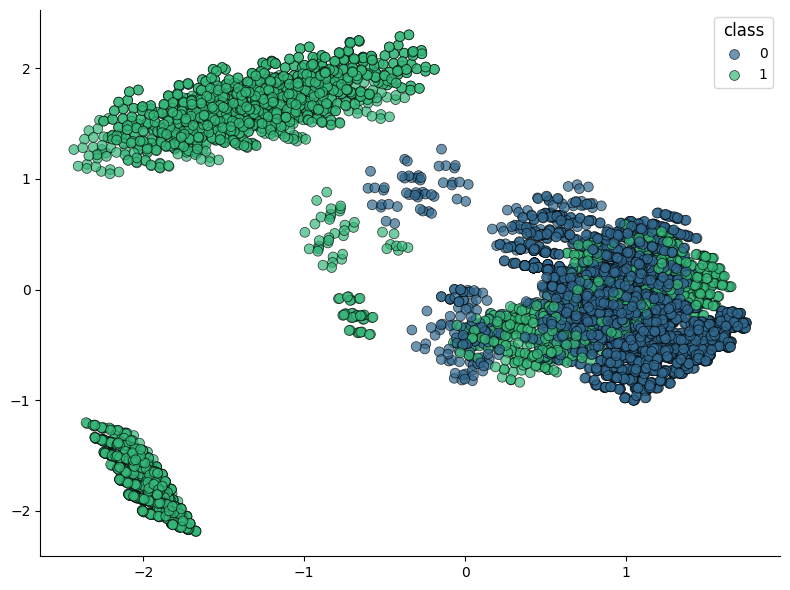
\includegraphics[width=\textwidth]{figures/mushroom_our_pca.png}
        \caption{Reduced Mushroom dataset}
        \label{our_pca_mushroom}
    \end{subfigure}
    \hfill
    % Segunda subfigura
    \begin{subfigure}[b]{0.45\textwidth}
        \centering
        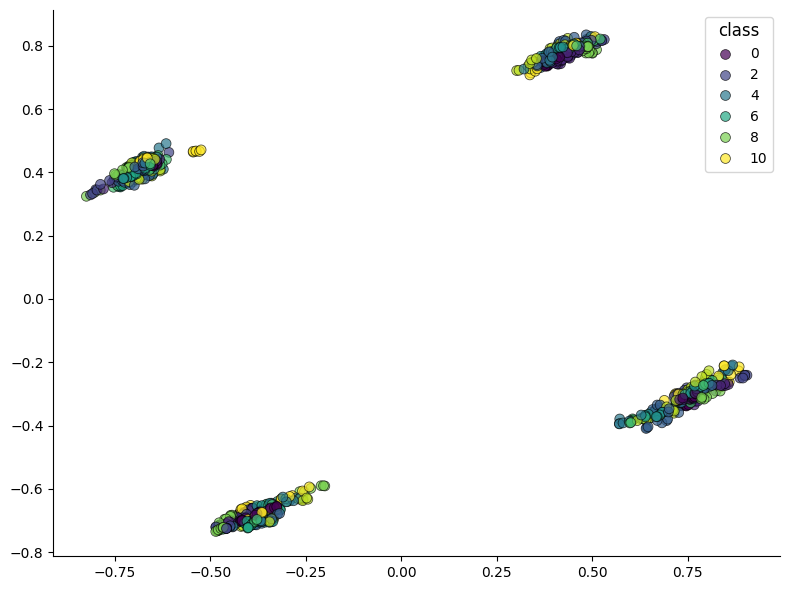
\includegraphics[width=\textwidth]{figures/vowel_our_pca.png}
        \caption{Reduced Vowel dataset}
        \label{our_pca_vowel}
    \end{subfigure}
    
    \caption{Visualization of the reduced datasets using our PCA implementation.}
    \label{fig:our_pca_datasets}
\end{figure}


\subsection{Our PCA vs sklearn.decomposition.PCA}
\label{subsec:pca-vs-scikit-pca}



\begin{figure}[h!]
    \centering
    % Primera subfigura
    \begin{subfigure}[b]{0.45\textwidth}
        \centering
        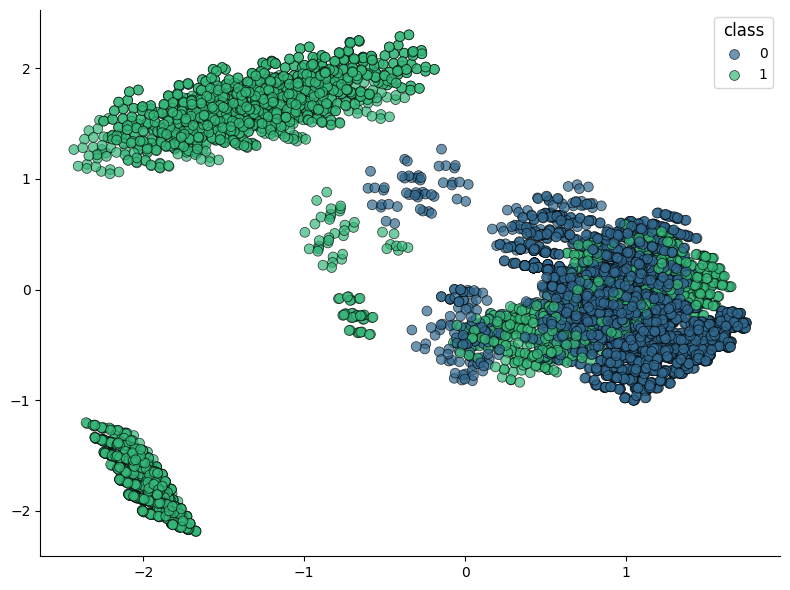
\includegraphics[width=\textwidth]{figures/mushroom_sklearn_pca.png}
        \caption{Reduced Mushroom dataset}
        \label{subfig:mushroom_sklearn_pca}
    \end{subfigure}
    \hfill
    % Segunda subfigura
    \begin{subfigure}[b]{0.45\textwidth}
        \centering
        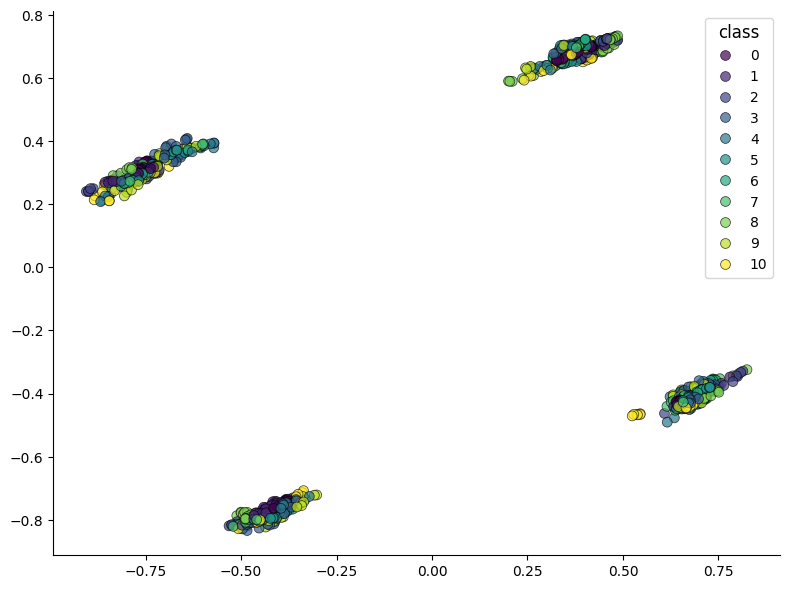
\includegraphics[width=\textwidth]{figures/vowel_sklearn_pca.png}
        \caption{Reduced Vowel dataset}
        \label{subfig:vowel_sklearn_pca}
    \end{subfigure}
    
    \caption{Visualization of the reduced datasets using Scikit-learn basic PCA.}
    \label{fig:sklearn_pca_datasets}
\end{figure}

The visualization compares the reduced datasets obtained using our custom PCA implementation (Figure \ref{fig:our_pca_datasets}) 
with those derived from the Scikit-learn PCA implementation (Figure \ref{fig:sklearn_pca_datasets}).
Both methods produce qualitatively similar results, preserving the overall structure and class separability of the datasets.
In the Mushroom dataset (subplots \ref{subfig:mushroom_sklearn_pca}), the two main clusters corresponding to the two classes are clearly distinguishable in both implementations,
indicating consistency in dimensionality reduction. For the Vowel dataset (subplots \ref{subfig:vowel_sklearn_pca}),
the distribution of the reduced data points aligns closely between the two approaches, with clusters for different classes exhibiting comparable orientations and separations.



% The results from the comparison between the project's PCA implementation and the scikit PCA implementation can be seen in Table \ref{tab:pca-vs-scikit-pca}.

% \begin{table}[h]
%     \centering
%     \begin{tabular}{|c|c|c|}
%         \hline
%         & \textbf{Project PCA} & \textbf{Scikit PCA} \\ \hline
%         \textbf{Performance} & 0.005s & 0.002s \\ \hline
%         \textbf{Memory usage} & 0.0001 MB & 0.0001 MB \\ \hline
%     \end{tabular}
%     \caption{Comparison between the project's PCA implementation and the scikit PCA implementation.}
%     \label{tab:pca-vs-scikit-pca}
% \end{table}

% The scikit PCA implementation is faster than the project's PCA implementation, but the difference in performance is not significant. The memory usage of both implementations is the same.


\subsection{Our PCA vs sklearn.decomposition.IncrementalPCA}
\label{subsec:pca-vs-incremental-pca}


\begin{figure}[h!]
    \centering
    % Primera subfigura
    \begin{subfigure}[b]{0.45\textwidth}
        \centering
        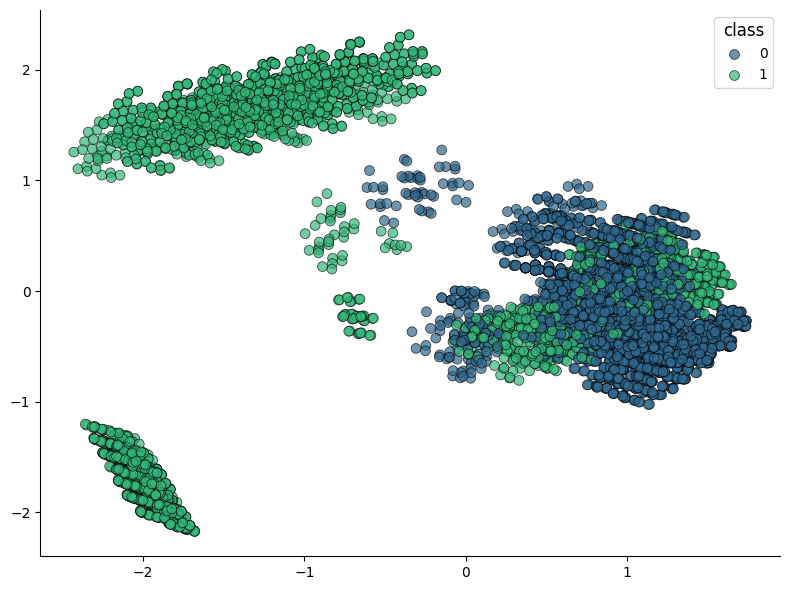
\includegraphics[width=\textwidth]{figures/mushroom_incremental_pca.png}
        \caption{Reduced Mushroom dataset}
        \label{subfig:mushroom_incremental_pca}
    \end{subfigure}
    \hfill
    % Segunda subfigura
    \begin{subfigure}[b]{0.45\textwidth}
        \centering
        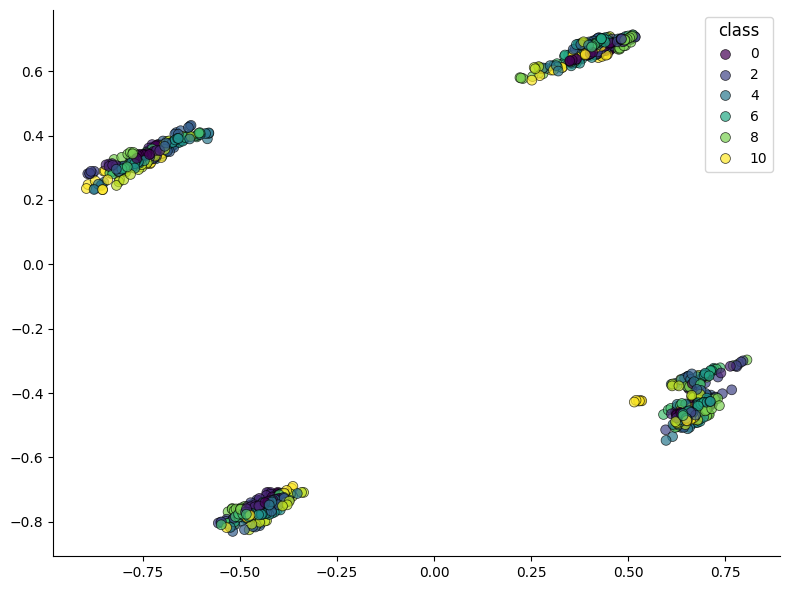
\includegraphics[width=\textwidth]{figures/vowel_incremental_pca.png}
        \caption{Reduced Vowel dataset}
        \label{subfig:vowel_incremental_pca}
    \end{subfigure}
    
    \caption{Visualization of the reduced datasets using Incremental PCA.}
    \label{fig:incremental_pca_datasets}
\end{figure}

The visualization compares the reduced datasets obtained using our custom PCA implementation (Figure \ref{fig:our_pca_datasets}) with those derived from Incremental PCA (Figure ]\ref{fig:incremental_pca_datasets}).
Both methods effectively capture the structure of the data, preserving the class separability in the reduced dimensionality space.
In the Mushroom dataset (subplots \ref{subfig:mushroom_incremental_pca}), the clustering of the two classes remains consistent between the two approaches, 
with both implementations producing similar geometric distributions. For the Vowel dataset (subplots \ref{subfig:vowel_incremental_pca}), 
Incremental PCA closely aligns with the results from our PCA implementation, maintaining the orientation and separation of class clusters.
This indicates that both methods achieve comparable results despite differences in computation techniques,
with Incremental PCA being particularly advantageous for large datasets where memory efficiency is critical.
The similarity in the visual outcomes demonstrates the reliability of our PCA implementation and its ability to replicate 
the performance of advanced techniques like Incremental PCA.

